
%!TEX root = edance.tex
\chapter{Frequency Response of Amplifiers}



\graphicspath{{./figs_freq_resp/}}



\subsection{Chapter Preview}

In this chapter we'll be looking at various techniques to calculate the frequency response of an amplifier.  We begin by reviewing the MOS transistor parasitics, and discuss passband and DC coupled amplifier response.  Next we use AC analysis to find the poles and zeros of the common source amplifier transfer function and discover that it's actually quite complicated, even for a system with two nodes.  We will introduce approximations and techniques that allow us to estimate the dominant poles in the frequency response.  The Miller approach allows us to get rid of pesky coupling capacitors that complicate the analysis, and most importantly, it will give us insights on when we must account for these capacitors and when we can ignore them.  Finally, the method of \emph{Open Circuit Time Constants} is a great way to analyze a complicated circuit with many capacitors, and we'll learn this technique in detail.  
 
\section{Frequency Response General Considerations}

For any circuit transfer function, the number of poles is a property of the circuit, and does not depend on the choice of input/output terminals.  The number of poles is given by the number of independent capacitors and inductors.  The zeros, on the other hand, depends on the transfer function, in other words the choice of the input and output ports.  In this chapter we will be pursuing techniques to discover the poles of an amplifier.  

\begin{figure}[tb]
\begin{center}
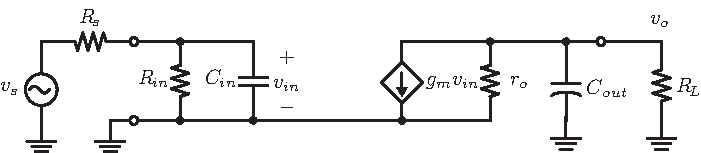
\includegraphics[scale=1]{amp_two_poles}
\end{center}
\caption{A generic transconductance amplifier with input capacitance $C_{in}$ and output capacitance $C_{out}$ at the input and output nodes.} \label{fig:amp_two_poles_indep}
\end{figure}

In many cases, the poles are actually easy to find and can be done by ``inspection".  Consider the example shown in Fig.~\ref{fig:amp_two_poles_indep}, consisting of an input capacitance $C_{in}$ and an output capacitance $C_{out}$.  We expect the circuit to have two poles, and we can almost read-off the poles by noting the input capacitance forms a low-pass filter.  The input pole is given by the $1/R_{eq}C_{in}$, where $R_{eq}$ is the equivalent resistance seen by the input capacitance.  To see this, note that
%
\begin{equation}
	v_{in} = \frac{Z_{in}}{Z_{in} + R_s} v_s \label{eq:vin}
\end{equation} 
%
where $Z_{in}$ is given by
%
\begin{equation}
	Z_{in} = \frac{R_{in}}{1 + j\omega R_{in} C_{in}}
\end{equation}
%
Substitution of this transfer function into Eq.~\ref{eq:vin} results in
%
\begin{equation}
	v_{in} = \frac{R_{in}}{R_{in} + R_s(1 + j\omega R_{in} C_{in})} v_s 
\end{equation}
%
Simplifying the transfer function, it's clear that the pole is due to $C_{in}$ and the parallel combination of $R_s $ and $R_{in}$:
%
\begin{equation}
	v_{in} = v_s \frac{R_{in}}{R_{in} + R_s} \frac{1}{ 1 + j\omega R_s || R_{in} C_{in}} 
\end{equation}
%
Likewise, if we examine the output of the amplifier, we note that output current flows into an impedance $Z_{out}$, which has a pole at a frequency given by $1/R_{out}C_{out}$, where $R_{out}$ is the equivalent resistance seen by $C_{out}$.  To show this, we again write the full transfer function:
%
\begin{equation}
	v_o = -g_m v_{in} Z_{out} 
\end{equation}
%
where $Z_{out}$ is given by
%
\begin{equation}
	Z_{out} = \frac{r_o || R_L}{1 + j\omega C_{out} r_o || R_L}
\end{equation}
%
Putting these results together, we have two independent poles, one from the input and one from the output:
%
\begin{equation}
	\frac{v_o}{v_s} = -g_m v_{in} Z_{out} = \frac{R_{in}}{R_{in} + R_s} \frac{-g_m r_o || R_L}{(1 + j\omega C_{out} r_o || R_L)(1 + j\omega R_s || R_{in} C_{in})}
\end{equation}
%
You should learn to identify these independent poles in the transfer function of amplifiers.  This will save you a lot of time and give you a first order solution to many problems.  What we cover for the rest of the chapter are poles that arise from ``coupling" capacitors, which couple charge from one node to another. These capacitors are ``pesky" and require special attention.


\section{Review MOS Parasitic Capacitors}

Recall that a MOS device has many internal capacitors that we've been ignoring up to now when calculating the low-frequency or pass-band response.  As shown in Fig.~\ref{fig:mos_caps_xsect}a, these capacitors are both intrinsic to the operation of the device, such as $C_{ox}$, or are present due to parasitic junctions and overlap/fringing between metals and contacts and the source/drain.  In the saturation region, we calculate the value of each capacitor and use the AC small-signal model, such as the three-terminal version shown in Fig.~\ref{fig:mos_caps_xsect}b.

%\begin{equation}
%	C_{gs} = \frac{2}{3} W L C_{ox} + L_{ov} W C_{ox}  
%\end{equation} 
%\begin{equation}
%	C_{gd} = C_{ov} + C_{\text{fringe}} = L_{ov} W C_{ox} + C_{\text{fringe}}
%\end{equation}
%\begin{equation}
%   C_{sb} = \frac{C_{j0}}{\sqrt{ 1 + V_{SB}/|\phi_b}}  A_{s,j} + \frac{C_{jsw0}}{\sqrt{ 1 + V_{SB}/|\phi_b}} P_{s,j}
%\end{equation}
%\begin{equation}
%   C_{db} = \frac{C_{j0}}{\sqrt{ 1 + V_{SB}/|\phi_b}}  A_{d,j} + \frac{C_{jsw0}}{\sqrt{ 1 + V_{SB}/|\phi_b}} P_{d,j}
%\end{equation}



\begin{figure}[tb]
\begin{center}
\begin{tabular}{cc}
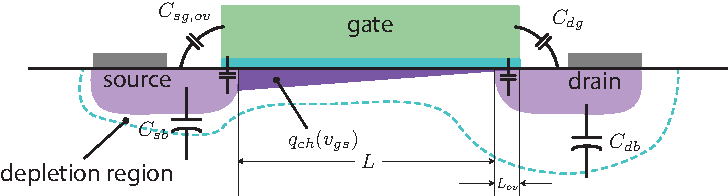
\includegraphics[width=.5\columnwidth]{mos_caps_xsect} &
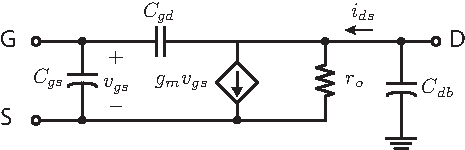
\includegraphics[width=.5\columnwidth]{mos3term_ac.pdf} \\
(a) & (b)\\
\end{tabular}
\end{center}
\caption{(a) Cross section of a MOS transistor in saturation and (b) the small-signal model including device capacitors.} \label{fig:mos_caps_xsect}
\end{figure}




\section{Common-Source Amplifier Frequency Response}


\subsection{Common Source Amplifier:  De-Coupling and Coupling Capacitors}

\begin{figure}[tb]
\begin{center}
\begin{tabular}{cc}
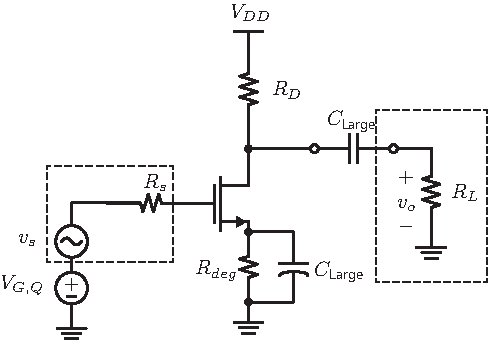
\includegraphics[width=.5\columnwidth]{cs_amp_acdc_RC_degen} &
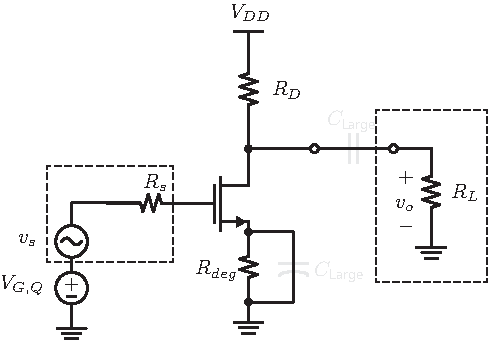
\includegraphics[width=.5\columnwidth]{cs_amp_acdc_RC_degen_capsshorted} \\
(a) & (b) \\
\end{tabular}
\end{center}
\caption{(a) Complete schematic of a discrete common source amplifier including biasing elements.  (b) AC equivalent circuit at mid-band frequencies.} \label{fig:cs_amp_acdc_RC_degen_capsshorted}
\end{figure}
 
Let's revisit the common-source amplifier, shown in Fig.~\ref{fig:cs_amp_acdc_RC_degen_capsshorted}a.  Since the load is referenced to ground, we cannot connect it directly to the transistor (without adversely affecting the operating point) so a large coupling capacitor is used.  Also, $R_{deg}$ is used for biasing the transistor but it impairs the gain, so it is ``bypassed" as well.  Note that the large coupling capacitors (degeneration and coupling) are shorts at AC frequencies, and can be neglected when calculating the passband and high-frequency response, as shown in Fig.~\ref{fig:cs_amp_acdc_RC_degen_capsshorted}b.



\subsection{Typical Passband Frequency Response}

\begin{figure}[tb]
\begin{center}
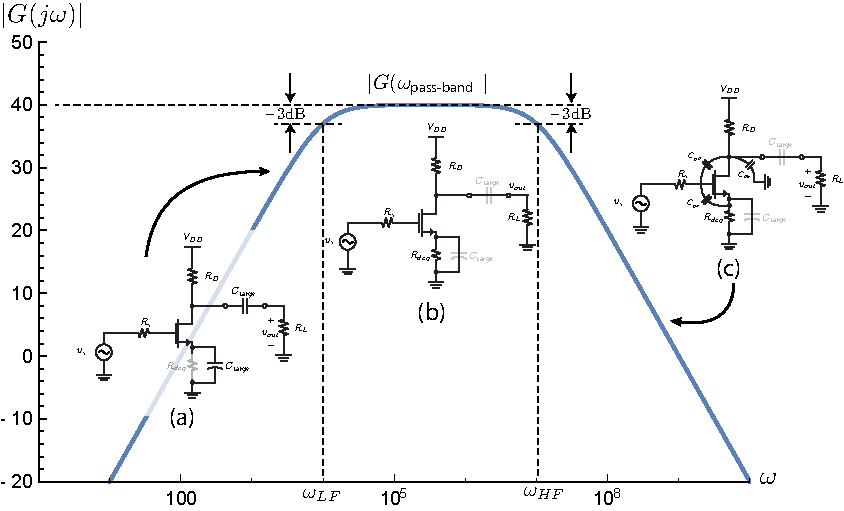
\includegraphics[width=.95\columnwidth]{amp_bandpass_decorate} 
\end{center}
\caption{The bandpass response of a common source amplifier highlighting the various regions and the circuit elements that dominate the frequency response.  (a) At low frequencies, small capacitors are open but large capacitors result in zeros in the transfer function.  (b) In the mid-band, the large capacitors are modeled as shorts and finally (c) in the high frequency region, small capacitors begin to play a role and determine the frequency roll-off characteristics.} \label{fig:amp_bandpass}
\end{figure}

In Fig.~\ref{fig:amp_bandpass}, we see a plot of a typical amplifier transfer functions, such as the common source discussed earlier.  We have a bandpass response, with a relatively flat region over a range of AC frequencies, and gain drop-off at both low and high frequencies.  Large coupling capacitors kill the gain at low frequencies and then high frequency poles reduce the gain at higher frequencies. Our goal for this chapter is to find the high frequency poles.  Mostly we will use techniques that give us the \emph{dominant} pole for multi-stage amplifiers, or the lowest frequency pole that gives rise to the high frequency roll-off.


\begin{figure}[tb]
\begin{center}
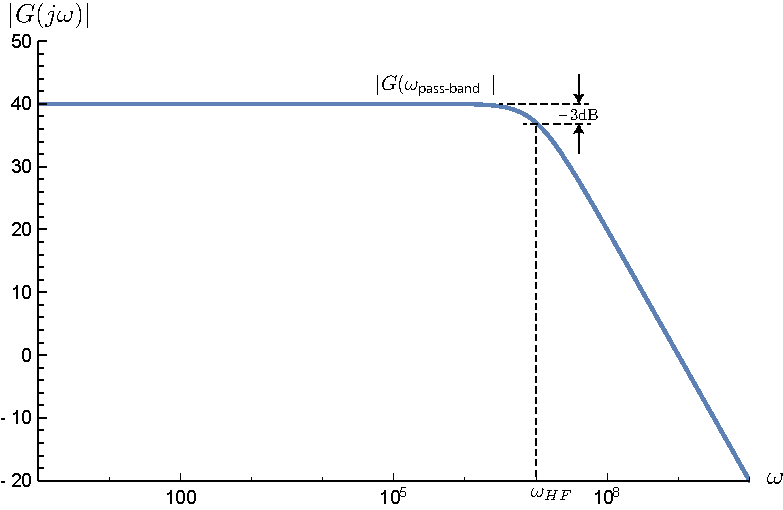
\includegraphics[width=.75\columnwidth]{amp_dccoup} 
\end{center}
\caption{A DC coupled amplifier frequency response is low-pass in nature and is characterized by high frequency poles that cause the transfer function to roll-off.} \label{fig:amp_dccoup}
\end{figure}



In a DC coupled amplifier response shown in Fig.~\ref{fig:amp_dccoup}, the gain does \textit{not} fall off at low frequencies, and the midband gain extends down to zero frequency. This is very desirable and we prefer DC coupled amplifiers over AC coupled ones.  The issue is that we have to ensure that the DC bias points of cascaded amplifiers are well matched.  In Chapter~\ref{ch:diffamps} we will study differential amplifiers that function over a wide range of DC voltages, allowing us to cascade the amplifiers without using large AC coupling capacitors.
 





\subsection{Common-Source Voltage Amplifier}


\begin{figure}[tb]
\begin{center}
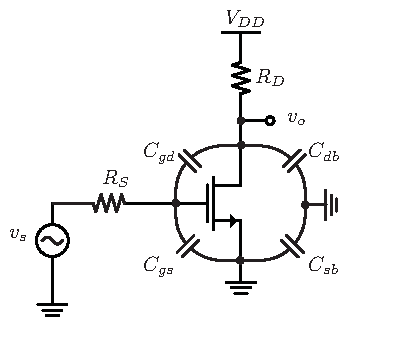
\includegraphics[scale=1]{cs_amp_caps}
\end{center}
\caption{The AC schematic of a common source amplifier with device capacitors.} \label{fig:cs_amp_caps}
\end{figure}

The AC model of the common-source amplifier, shown in Fig.~\ref{fig:cs_amp_caps}, has many capacitors.  
 $C_{sb}$ is connected to ground on both sides, therefore it can be ignored.  The small-signal model, shown in Fig.~\ref{fig:cs_amp_ac_caps}, has two nodes.  Note that we cannot solve this problem by inspection, as we did for the circuit of Fig.~\ref{fig:amp_two_poles_indep}, because of the presence of the capacitance $C_{gd}$. We can solve problem directly by nodal analysis, and this is a good approach if the circuit is ``small".  This will lead to the complete transfer function of the circuit.
 



\section{Common-Source:  Brute Force Frequency Response Calculation}




\begin{figure}[tb]
\begin{center}
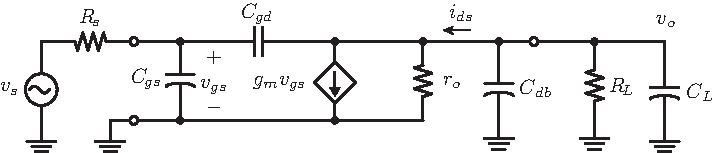
\includegraphics[scale=1]{cs_amp_ac_caps}
\end{center}
\caption{Small-signal model of a common source amplifier with device capacitors and load capacitance.} \label{fig:cs_amp_ac_caps}
\end{figure}

So let's try to analyze the transfer function, as it only has two nodes.  This looks ``easy", but don't forget that every capacitor leads to a pole.  With three capacitors present, we're dealing with a cubic transfer function! For now we will ignore $C_{db}+C_L$ to simplify the math to a second order transfer function.  

Let $R'_L = r_o || R_L$ and write KCL at each node of the circuit:
%
\begin{equation}
	\frac{v_{gs} - v_s}{R_s} + s C_{gs} v_{gs} + (v_{gs} - v_o) s C_{gd} = 0
\end{equation}
%
\begin{equation}
	\frac{v_o}{R'_L} + g_m v_{gs} + (v_o - v_{gs}) s C_{gd} = 0 
\end{equation}
%
Let's combine these two equations into a matrix:
%
\begin{equation}
	\begin{pmatrix}
	1 + s R_s (C_{gs} + C_{gd}) & -s C_{gd} R_s \\
	g_m R'_L - s C_{gd} R'_L & 1 + s R'_L C_{gd}  \\
	\end{pmatrix}
	 \begin{pmatrix}
		v_{gs} \\ v_o \\
	\end{pmatrix} 	
	=
	 \begin{pmatrix}
		v_s \\ 0 \\
	\end{pmatrix} 
\end{equation}
%
Using Cramer's Rule or another approach, it's easy to show that the transfer function is given by
%
\begin{equation}
	v_o = \frac{-g_m R'_L (1 - \frac{s C_{gd}}{g_m})}
	{1 + s \left( R'_L C_{gd} + R_s (C_{gs} + C_{gd}) + R_s C_{gd} g_m R'_L \right) 
	+ s^2 (R'_L R_s C_{gd} C_{gs}) } v_s
\label{eq:exact_transfer}
\end{equation}
To check this result, let's examine the low-frequency gain:
%
\begin{equation}
\frac{{{v_{o}}}}{{{v_{s}}}}(s = 0) = \frac{{ - {g_m}\left( {{r_o}||{R_L}} \right)\left( {1 - j0} \right)}}{{\left( {1 + j0 + (j0)(j0)} \right) }} =  - {g_m}\left( {{r_o}||{R_L}} \right)
\end{equation}
This result is consistent with our previous analysis of the midband gain.  Note that transfer function has a zero, a frequency that causes the transfer function to go to zero:
%
\begin{equation} 
	{\omega_z} = \frac{g_m}{C_{gd}}
\end{equation}
%
The origin of this zero is due to the feedthrough capacitor $C_{gd}$ which adds a signal to the output with opposite phase as the $g_m$, and so at a high enough frequency, this feed-forward current cancels the gain of the amplifier.
%

We would like to put the transfer function into the following form:
%
\begin{equation}
\frac{v_{o}}{v_{s}} = 
	\frac{ - g_m \left( r_o||R_L \right) \left( 1 - j\omega /\omega_z \right)}
	{\left( 1 + j\omega /\omega_{p1} \right) \left( 1 + j\omega /\omega_{p2} \right) }
\end{equation}
%
Since the denominator of transfer function is second order, we can solve it exactly with the quadratic formula, but the results are messy.  We'll make an approximation that the poles are widely separated, in other words $\omega_{p1} \ll \omega_{p2}$.  This approximation is valid in most circumstances and leads to a simpler result that we'll use:
%
\begin{equation}
\frac{v_{o}}{v_{s}} = 
	\frac{ - g_m \left( r_o||R_L \right) \left( 1 - j\omega /\omega_z \right)}
	{ 1 + j\omega \left( 1/\omega_{p1} +  1/\omega_{p2} \right) + (j\omega)^2 / (\omega_{p1}\omega_{p2})   }
	\approx 
	\frac{ - g_m \left( r_o||R_L \right) \left( 1 - j\omega /\omega_z \right)}
	{ 1 + j\omega \left( 1/\omega_{p1}  \right) + (j\omega)^2 / (\omega_{p1}\omega_{p2})   }
\end{equation}
%
This approximation allows us to quickly estimate the ``dominant" pole by equating the above equation with \ref{eq:exact_transfer}:
%
\begin{equation} 
{\omega _{p1}} \approx \frac{1}{{{R_s}\left\{ {{C_{gs}} + \left( {1 + {g_m}{{R}_{o}}} \right){C_{gd}}} \right\} + {{R}_{o}}{C_{gd}}}}  \label{eq:pole_almost_exact}
\end{equation}
%
The result is not exact, since we neglected $C_L$ and $C_{db}$, and provides little insight.  These poles are calculated after doing a lot of algebraic manipulations on the transfer function, even though we're only dealing with a second order transfer function. There must be an easier and better way!
 

\section{The Miller Theorem}

\subsection{The Miller Effect}

\begin{figure}[tb]
\begin{center}
\begin{tabular}{cc}
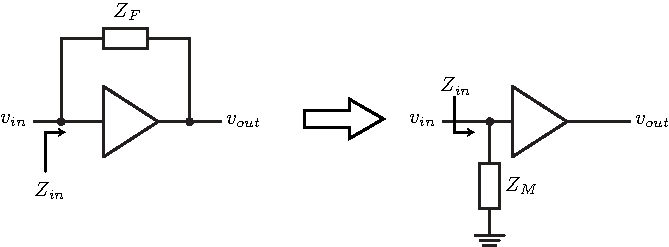
\includegraphics[scale=.9]{miller2} &
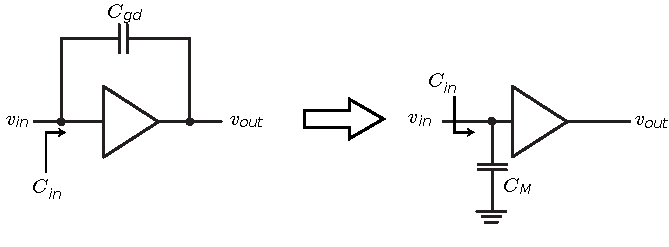
\includegraphics[scale=.9]{miller_cap} \\
(a) & (b)  \\
\end{tabular}
\end{center}
\caption{(a) The Miller Theorem allows us to replace an impedance $Z_F$ coupling two nodes with a simpler impedance to ground $Z_M$.  (b) This is particularly useful for analyzing the frequency response of an amplifier when coupling capacitors such as $C_{gd}$ appear.} \label{fig:miller1}
\end{figure}


Consider an ideal amplifier with gain $A$ and a feedback impedance $Z_F$ from input to output shown in Fig.~\ref{fig:miller1}a.  Let's calculate the input impedance of this circuit assuming the amplifier has infinite input impedance.  In that case, the only current flow is due to $Z_F$:
%
\begin{equation}
	i_{in} = \frac{v_{in} - v_{out}}{Z_F}
\end{equation}
%
Since the output is a scaled copy of the input:
%
\begin{equation}
	i_{in} = \frac{ v_{in} - A\cdot v_{in} }{Z_F}
\end{equation}
%
Notice that the above equation only involves the input node.  We can therefore pretend the current flows to ground as shown in Fig.~\ref{fig:miller1}a:
%
\begin{equation}
	i_{in} = \frac{v_{in}}{\frac{Z_F}{1 - A}}
\end{equation}
% 
In other words, we can replace the feedback $Z_F$ with a (smaller) impedance to ground (assuming A is negative):
%
\begin{equation}
	Z_M = \frac{Z_F}{1 - A}
\end{equation}
%
If this seems like a ``sleight of hand", keep in mind that in practice $Z_F$ will also affect the gain $A$, so technically we don't really know $A$. The trick is to estimate $A$, especially when the gain is not a strong function of $Z_F$.



\subsection{The Miller Effect of a Capacitor}

Applying the Miller Theorem to a capacitor, shown in Fig.~\ref{fig:miller1}b, we have a capacitor that couples two notes.  In this case, it's across an inverting amplifier, and so the effective capacitance is boosted:
%
\begin{equation}
	Z_M = \frac{1}{j\omega C_M} = \frac{\frac{1}{j\omega C_{gd}}}{ 1 - A}
\end{equation}
%
For example, in a common-source amplifier, the capacitor is $C_{gd}$, the pesky capacitor that complicated our analysis of the frequency response.  Applying the Miller Theorem to the capacitive impedance: 
\begin{equation}
	Z_M = \frac{1}{j\omega C_{gd} (1 - A)}
\end{equation}
%
This implies that we can replace $C_{gd}$ with a capacitor at the input to ground of larger magnitude:
%
\begin{equation}
	C_{in} = C_M  = C_{gd} (1-A)
\end{equation}
%
Note that for a common-source amplifier $A$ is negative, so the overall capacitance is positive.  If the voltage gain is large, then the capacitance is boosted to a much larger value to ground.  The physical reason is not too difficult to understand if you consider that in a capacitor current flows due to the rate of change of the voltage difference  across the capacitor.  An amplifier with negative gain will boost this voltage difference, causing one terminal to move with a much larger amplitude compared to the other, and a correspondingly larger input current is drawn. 




\section{Common-Source:  Miller Approach Frequency Response Calculation}



\begin{figure}[tb]
\begin{center}
\begin{tabular}{cc}
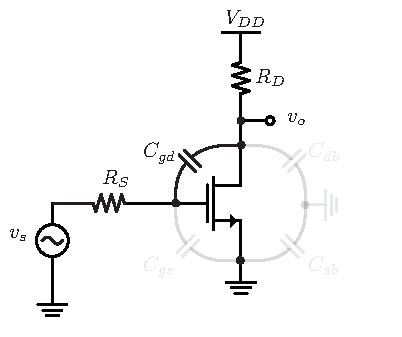
\includegraphics[scale=1]{cs_amp_cgd} &
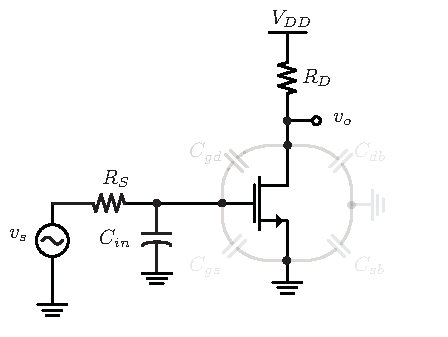
\includegraphics[scale=1]{cs_amp_cgd_miller} \\
(a) & (b) \\
\end{tabular}
\end{center}
\caption{(a) In a common source amplifier, $C_{gd}$ is the most difficult capacitor to account for as it couples two nodes.  (b) Using the Miller Theorem, we replace it with an equivalent input capacitance $C_{in}$. } \label{fig:cs_amp_cgd}
\end{figure}


Now we apply the Miller Theorem to the $C_{gd}$ feedback capacitor in the MOS amplifier, shown in Fig.~\ref{fig:cs_amp_cgd}:  
% 
\begin{equation}
{C_{in}} = \frac{1}{{j\omega {C_{M}}}} = \left( {\frac{1}{{1 - {A_{v,Cgd}}}}} \right)\left( {\frac{1}{{j\omega {C_{gd}}}}} \right) = \frac{1}{{j\omega \left[ {\left( {1 - {A_{vCgd}}} \right){C_{gd}}} \right]}}
\end{equation}
%
Using this input capacitance, we modify the small-signal model as shown in Fig.~\ref{fig:cs_amp_ac_caps_miller}.  This circuit is much simpler than the original amplifier since the coupling capacitor is removed and the two nodes are seemingly independent.   The only trouble is that $A_{vCgd}$ is not known exactly but we take the low-frequency value as an approximation:
%
\begin{equation}
	A_{vCgd} \approx -g_m R_{o}
\end{equation}
%
Using the Miller approximation result, we calculate the $RC$ time constant of the input pole by inspection:
%
\begin{equation}
	{\omega _{p1}}^{ - 1} = {R_s}\left[ {{C_{gs}} + \left( {1 + {g_m}{{R}_{o}}} \right){C_{gd}}} \right]
\end{equation}
%
If we compare this to the previously derived result, we have:
%
\begin{equation} 
	{\omega _{p1}}^{ - 1} = {R_s}\left[ {{C_{gs}} + \left( {1 + {g_m}{{R}_{o}}} \right){C_{gd}}} \right] + {R'_{L}}{C_{gd}}
\end{equation}
The results are very close except for the last term, which usually does not dominate.  The Miller effect is much simpler and as an added bonus, it gives us insight into the  gain-bandwidth trade-off of the amplifier.  If we boost the gain of the common-source amplifier, the input pole drops.  This is one of the main limitations of a common source amplifier, something we'll address later when we discuss multi-stage amplifiers.


\begin{figure}[tb]
\begin{center}
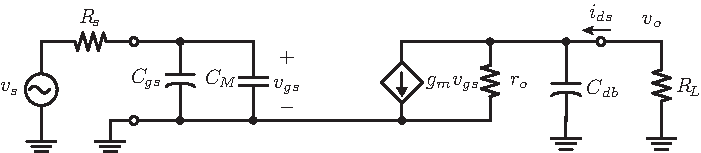
\includegraphics[scale=1]{cs_amp_ac_caps_miller}
\end{center}
\caption{Small-signal model of a common source amplifier with $C_{gd}$ replaced by a Miller capacitor $C_M$.} \label{fig:cs_amp_ac_caps_miller}
\end{figure}

 





\section{Common Drain Amplifier Frequency Response}




\begin{figure}[tb]
\begin{center}
\begin{tabular}{cc}
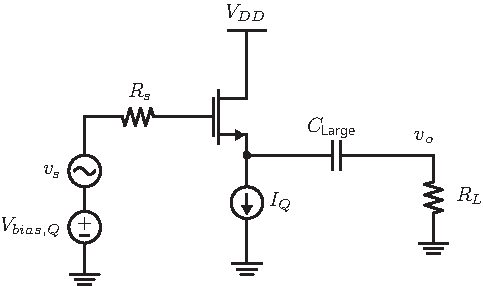
\includegraphics[scale=.8]{cd_amp_load} &
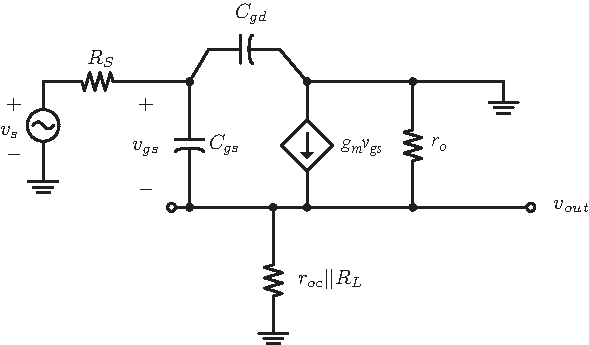
\includegraphics[scale=.8]{cd_amp_ss_cap} \\
(a) & (b) \\
\end{tabular}
\end{center}
\caption{(a) Schematic of a common drain amplifier.  (b) Small-signal AC model of the common drain amplifier.} \label{fig:cd_amp_load}
\end{figure}

Let's now compute the bandwidth of a common drain amplifier, also known as the source follower, shown in Fig.~\ref{fig:cd_amp_load}.  We can replace the current source with MOSFET-based current mirror, and we simply model it by $r_{oc}$.  In the small-signal model with capacitors shown in Fig.~\ref{fig:cd_amp_load}b, we use the DC small-signal gain and the Miller effect to calculate the input capacitance.  This will allow us to estimate the dominant pole.
 



\subsection{Voltage Gain Across $C_{gs}$}

%\begin{figure}[tb]
%\begin{center}
%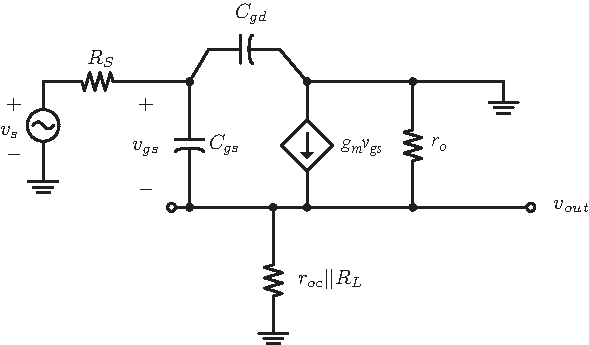
\includegraphics[scale=1]{cd_amp_ss_cap}
%\end{center}
%\caption{cd amp ss cap} \label{fig:cd_amp_ss_cap}
%\end{figure}

Note that the Miller capacitor in this case is $C_{gs}$, the gate-source capacitor is between the input and output.  Recall the gain of a common drain amplifier:
%% 
%\begin{equation}
%	\frac{{{v_{out}}}}{{\left. {{r_o}} \right\|{r_{oc}}}} = {g_m}{v_{gs}} = {g_m}({v_{in}} - {v_{out}})
%\end{equation}
%Collecting terms:
%\begin{equation}
%	{v_{out}}\left( {\frac{1}{{\left. {{r_o}} \right\|{r_{oc}}}} + {g_m}} \right) = {g_m}{v_{in}}
%\end{equation}
%%
%We find the voltage gain across the capacitor:
%%
\begin{equation}
	\frac{{{v_{out}}}}{{{v_{in}}}} = \frac{{{g_m}}}{{\left( {\frac{1}{{\left. {{r_o}} \right\|{r_{oc}}}} + {g_m}} \right)}} = \frac{{{g_m}(\left. {{r_o}} \right\|{r_{oc}})}}{{1 + {g_m}(\left. {{r_o}} \right\|{r_{oc}})}} = {A_{vCgs}}
\end{equation}
%
We can therefore replace the capacitance at the input with an effective capacitance:
%
\begin{equation} 
	{C_{in}} = {C_{gd}} + {C_M} 
\end{equation}
%
where $C_M$ is the Miller multiplied capacitor $C_{gs}$:
%
\begin{equation} 
	{C_{in}} = {C_{gd}} + (1 - {A_{v{C_{gs}}}}){C_{gs}} 
\end{equation}
%
If we substitute the low-frequency gain $A_{v{C_{gs}}}$:
%
\begin{equation} 
	{C_{in}} = {C_{gd}} + \left(1 - \frac{{{g_m}(\left. {{r_o}} \right\|{r_{oc}})}}{{1 + {g_m}(\left. {{r_o}} \right\|{r_{oc}})}} \right){C_{gs}}
\end{equation}
This can be simplified:
%
\begin{equation} 
	{C_{in}} = {C_{gd}} + \left(\frac{1}{{1 + {g_m}(\left. {{r_o}} \right\|{r_{oc}})}} \right){C_{gs}} 
\end{equation}
%
Notice that the second term is small if $g_m r_o || r_{oc}$ is large:
%
\begin{equation} 
	{C_{in}} \approx {C_{gd}} 
\end{equation}
%
What just happened?  The Miller capacitor nearly vanishes in this case, because it's ``bootstrapped", meaning the gain across the capacitor is nearly unity, and it has a positive sign, so very little current flows through it.



%\begin{figure}[tb]
%\begin{center}
%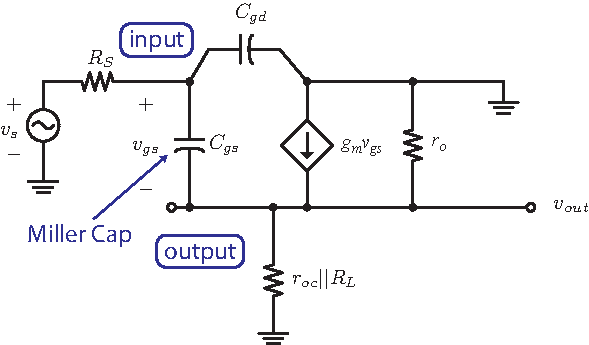
\includegraphics[scale=1]{cd_amp_ss_cap_miller}
%\end{center}
%\caption{cd amp ss cap miller} \label{fig:cd_amp_ss_cap_miller}
%\end{figure}

 
\subsection{Bandwidth of Source Follower}

The input low-pass filter’s –3 dB frequency is given by:
%
\begin{equation} 
	{\omega _p}^{ - 1} = {R_S}\left( {{C_{gd}} + \frac{{{C_{gs}}}}{{1 + {g_m}(\left. {{r_o}} \right\|{r_{oc}})}}} \right)
\end{equation}
%
Let's substitute some favorable values of $R_S$,$r_o$:
\begin{equation} 
	{R_S} \approx 1/{g_m} 
\end{equation}
\begin{equation} 
	{r_o} \gg 1/{g_m} 
\end{equation}
This gives:
\begin{equation} 
	{\omega _p}^{ - 1} \approx \left( {1/{g_m}} \right)\left( {{C_{gd}} + \frac{{{C_{gs}}}}{{1 + BIG}}} \right) \approx {C_{gd}}/{g_m} 
\end{equation}
If we simplify this, we see that:
\begin{equation}
	{\omega _p} \approx {g_m}/{C_{gd}}
\end{equation}
%
As we will shortly show, this is a very high frequency, much higher than the validity of our approximations and models.  The net result is the input pole is likely high impedance, especially if driven by a moderate source impedance.
 


\subsection{Miller Summary}


Let's summarize how the Miller effect played out in these two very different scenarios:

\begin{itemize}

\item Common source amplifier:  Miller multiplied capacitor has \underline{detrimental} impact.
%
\[
	A_v = \text{A large negative number, say -100} 
\]
%
\[	
	{C_{Miller}} = (1 - {A_{V,{C_{gd}}}}){C_{gd}} \approx 100{C_{gd}}
\]
%
\item Common drain amplifier:  ``Bootstrapped" capacitor has negligible impact on bandwidth.
%
\[
	A_v = \text{slightly less than unity and positive} 
\]
%
\[
	{C_{Miller}} = (1 - {A_{V,Cgs}}){C_{gs}} \simeq 0
\]

\end{itemize}
 

\section{Common Gate Amplifier Bandwidth}

The small-signal schematic of the common gate amplifier is shown in Fig.~\ref{fig:cg_amp_caps}. While there are four capacitors in the model, three are in parallel, so we only expect two poles.  Also notice that both $C_{gd}$ and $C_{gs}$ are grounded at one node, and so there are no input-to-output coupling capacitors, and hence no Miller effect for the capacitors.  This makes the common gate amplifier in general a broadband amplifier stage.  To see this, we'll analyze the circuit, first using an approximation, and then using the complete equations.  

\begin{figure}[tb]
\begin{center}
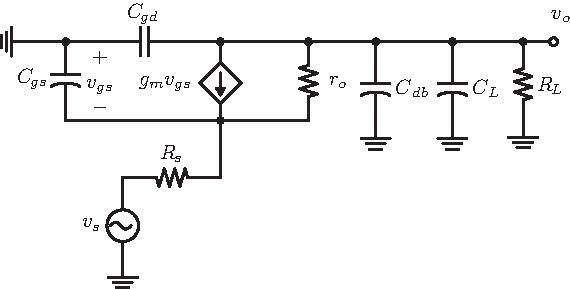
\includegraphics[scale=1]{amp_cg_ss}
\end{center}
\caption{Small-signal AC model of a common gate amplifier.  Note that even though there are no coupling capacitors from input to output, there is a coupling resistor $r_o$.} \label{fig:cg_amp_caps}
\end{figure}


To begin, observe that the resistor $r_o$ is coupled from the input to the output, and so we could apply the Miller theorem to this resistance.  What we'll find is that the impedance level at the input is low enough and dominated by the low impedance presented by the transistor, so neglecting $r_o$ does not change impedance levels appreciably.  In fact, if we ignore $r_o$ altogether, we'll find that the circuit consists of two independent nodes, and it's easily analyzed by inspection.

At the input, the pole arising from $C_{gs}$ can be estimated by finding the equivalent resistance seen at the input node, which is dominated by the transistor $1/g_m$ in parallel with $R_s$:
%
\begin{equation}
	\omega_1 = \frac{1}{C_{gs} R_s||\frac{1}{g_m}}
\end{equation}    
%
At the output node, the parallel combination of $C_L + C_{gd}$ sees a resistance of $R_L$ in parallel with a high impedance presented by the transistor, which we'll ignore:
%
\begin{equation}
	\omega_2 = \frac{1}{(C_{L} + C_{gd} + C_{db}) R_L}
\end{equation}    
%
The first pole can be lower bounded by:
%
\begin{equation}
	\omega = \frac{g_m}{C_{gs}}
\end{equation}
%
In the next section we'll show that this frequency is a device property known as the unity gain frequency and is usually a very high frequency for modern short channel devices biased in saturation.  The second pole depends on both the load capacitance and the load resistance, and component values can be selected to ensure sufficient bandwidth.

It's always good to verify our assumptions by performing a more complete analysis.  The nodal equations at the input and output are given by
%
\begin{equation}
	\begin{pmatrix}
	(G_s + g_m + g_o + s C_{gs})  & - g_o \\
	-(g_m + g_o) & (g_o + g_L + s C'_L)
	\end{pmatrix}
	\begin{pmatrix}
	v_1 \\ v_2 \\
	\end{pmatrix}
	=
	\begin{pmatrix}
	v_s G_s \\ 0 \\
	\end{pmatrix}	
\end{equation}
%
In writing these equations, we have used conductances $g_o = 1/r_o$, for example $G_s = 1/R_s$, and an effective load capacitance $C'_L = C_{gd} + C_{db} + C_L$.  We can easily solve this 2$\times$2 system to obtain
%
\begin{equation}
	v_2 = \frac{(g_m + g_o) G_s}
			   {(g_o + g_L + s C'_L)(G_s + g_m + g_o + s C_{gs}) + g_o (g_m + g_o)} v_s
\end{equation}
%
As expected, if we neglect the $g_o$ terms, we get a simple separable second-order system with an input pole and an output pole.  From the full equations, we can see why we are justified in neglecting $g_o$ as it always appears in sums with much larger conductances.  For example $g_m r_o \gg 1$ implies that $g_m \gg g_o$.  Let's first check the DC gain and verify it matches our previous calculations:
%
\begin{equation}
	\frac{v_2}{v_s}(s = 0) = 
		  \frac{(g_m + g_o) G_s}
			   {(g_o + g_L)(G_s + g_m + g_o) + g_o (g_m + g_o)} 
\end{equation}
%
This expression is complicated by the feedforward gain due to $g_o$.  Neglecting $g_o$ we have a simplified expression that matches our simpler calculations:
%
\begin{equation}
	\frac{v_2}{v_s}(s = 0) \approx \frac{g_m}{1 + g_m R_s} R_L 
\end{equation}
%
Finally, under the $g_o = 0$ approximation, the poles are given by:
%
\begin{equation}
	\omega_1 = \frac{G_s + g_m}{C_{gs}}
\end{equation}
%
and
%
\begin{equation}
	\omega_2 = \frac{G_L}{C'_{L}}
\end{equation}
%
which agree with our estimations, as expected.


\section{Device unity gain frequency $f_T$}

In the previous section, we encountered a lower bound for the common gate input pole:
%
\begin{equation}
	\omega = \frac{g_m}{C_{gs}}
\end{equation}
%
We claimed that this is a very high frequency.  To show this, we're going to define the unity-gain frequency $f_T$ of a transistor, a parameter that characterizes the high frequency performance of a transistor for analog circuits.



\subsection{Unity-Gain Frequency $f_T$}

\begin{figure}[tb]
\begin{center}
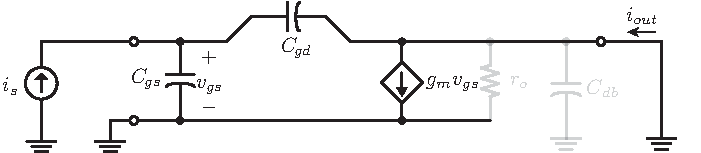
\includegraphics[scale=1]{hybrid_pi_ft}
\end{center}
\caption{AC schematic for calculation of the current gain of a MOS transistor.} \label{fig:hybrid_pi_ft}
\end{figure}

Let's calculate the current gain of a MOS transistor by shorting the output, as shown in the setup in Fig.~\ref{fig:hybrid_pi_ft}.  Note that the input $v_{gs}$ is given by:
\begin{equation}
	{v_{gs}} = \frac{{{i_s}}}{{s{C_{gs}} + s{C_{gd}}}}
\end{equation}
%
KCL at the output results in:
%
\begin{equation} 
	{i_{out}} + \frac{{{v_{gs}}}}{{1/s{C_{gd}}}} = {g_m}{v_{gs}} 
\end{equation}
This generates an output current:
%
\begin{equation} 
	{i_{out}} = {g_m}{v_{gs}} - s{C_{gd}}{v_{gs}} \approx {g_m}{v_{gs}} = {g_m}\frac{{{i_s}}}{{s{C_{gs}} + s{C_{gd}}}}
\end{equation}
%
The approximation is valid since the $g_m$ of a transistor should dominate over the parasitic feedthrough current through $C_{gd}$.  This means the current gain $A_i$ is given by:
%
\begin{equation} 
	{A_i} = \frac{{{i_{out}}}}{{{i_s}}} = \frac{{{g_m}}}{{s{C_{gs}} + s{C_{gd}}}} 
\end{equation}
Making the substitution $s = j\omega$ and taking the magnitude of the gain:
%
\begin{equation} 
	\left| {\frac{{{I_o}}}{{{I_i}}}} \right| = \frac{{{g_m}}}{{\omega ({C_{gs}} + {C_{gd}})}} 
\end{equation}
%
We define $\omega_T = 2\pi f_T$ as the unity gain frequency by equating the magnitude to unity and solving for $\omega_T$:
%
\begin{equation} 
	{\omega _T} = \frac{{{g_m}}}{{{C_{gs}} + {C_{gd}}}}   \label{eq:ft1}
\end{equation}
%
Substituting the small-signal parameters:
%
\begin{equation}
	C_{gs} = \frac{2}{3} W L C_{ox}
\end{equation}
%
\begin{equation}
	C_{gd} = \frac{2}{3} W \delta L C_{ox}
\end{equation}
%
\begin{equation}
	g_m = \mu C_{ox} \frac{W}{L} (V_{gs} - V_T)
\end{equation}
%
Substituting in Eq.~\ref{eq:ft1}, we have:
%
\begin{equation} 
	{\omega _T} = \frac{\mu \cancel{C_{ox}} \frac{\cancel{W}}{L} (V_{gs} - V_T)}
				 {\frac{2}{3} \cancel{W} (L + \delta L) \cancel{C_{ox}}} =
				 \frac{3}{2} \frac{\mu (V_{gs} - V_T)}
				 	{L(L+\delta L)}  \label{eq:ft2}
\end{equation}
%
There are some nice physical relations that we can invoke to explain this equation.  For example the term
%
\begin{equation}
	E_{sat} = \frac{(V_{gs} - V_T)}{L}
\end{equation}
%
is the average electric field in the channel of the transistor when biased in saturation, since $V_{ds,ch} = V_{gs} - V_T$ and so $\mu E_{sat}$ is the velocity of carriers.  This means that the overall expression is approximately the time it takes a carrier to cross the channel.  

As gate length reduces in advanced technology nodes, the $f_T$ increases.  Today we have devices $L < 100$nm and $f_T > 100$ GHz of unity gain frequency, so when we design amplifiers with bandwidths up to 100's of MHz, this unity gain frequency is quite high.

Why do we bother to define $f_T$?  It's an important limit not only for current amplifiers, but as we'll see later, it's actually the gain-bandwidth limit for all amplifiers, including voltage amplifiers.  We'll find that even with broadband amplifier stages, it's hard to beat the $f_T$ bandwidth.  In advanced analog design courses, you'll learn that  most amplifiers are limited in gain-bandwidth to about $f_T$. 





\subsection{Frequency Response of Multistage Amplifiers}

We have a \textit{systematic technique} to study amplifier performance (derive transfer function, study poles/zeros/Bode plots).  In most cases, the systematic approach is too cumbersome. We have a good qualitative understanding of circuit performance (e.g., CS suffers from Miller effect, CD and CG are wideband stages).  Next we will introduce the \textit{Open Circuit Time Constants} approach, which is an analytical technique capable of estimating  the dominant (lowest) pole for an amplifier with many capacitors.


\section{The Method of Open-Circuit Time Constants (OCTC)}



\subsection{OCTC Assumptions}

There are many assumptions that go into the analysis approach.  First, we assume the transfer function doesn't have \textit{zeros}.  We will also make a  \textit{dominant pole} approximation, in other words we assume that $\omega_1 \ll \min(\omega_2, \omega_3, \dots, \omega_n)$. Working with the all-pole transfer function:
% 
\begin{equation}
	H(j\omega ) = \frac{{{H_o}}}{{\left( {1 + j\omega {b_1} + {{(j\omega )}^2}{b_2} + {{(j\omega )}^3}{b_3} + ...} \right)}} 
	\label{eq:h1}
\end{equation}
%
If we factor the denominator:
% 
\begin{equation}
	H(j\omega ) = \frac{{{H_o}}}{{\left( {1 + j\omega /{\omega _1}} \right)\left( {1 + j\omega /{\omega _2}} \right)...\left( {1 + j\omega /{\omega _n}} \right)}}
\end{equation}
%
Now multiply out the denominator again:
%
\begin{equation}  
	H(j\omega ) \approx \frac{{{H_o}}}{{1 + j\omega \left( {\frac{1}{{{\omega _1}}} + \frac{1}{{{\omega _2}}} + ... + \frac{1}{{{\omega _n}}}} \right) + \cdots }}
\label{eq:h2}
\end{equation}
%
Equating \ref{eq:h1} and \ref{eq:h2}, and using $\omega_1 \ll \min(\omega_2, \omega_3, \dots, \omega_n)$, we have
% 
\begin{equation} 
	{b_1} = \frac{1}{{{\omega _1}}} + \frac{1}{{{\omega _2}}} + ... + \frac{1}{{{\omega _n}}} \approx \frac{1}{{{\omega _1}}}
\end{equation}
%
So if we can estimate $b_1$, we can also estimate the dominant pole.

\subsection{Procedure to Find $b_1$}

$b_1$ can be calculated as follows:  $b_1$ is the sum of \textit{open-circuit time constants} $\tau_i$ which can be found by considering each capacitor $C_i$ in the amplifier separately and finding its Thévenin resistance $R_{C_i}$.  Next we calculate the time-constant of each capacitor $\tau_i = R_{C_i} C_i$ and sum them together
%
\begin{equation}
	b_1 = \sum_{i=1}^n C_i R_{C_i} 
\end{equation}
%
and so
%
\begin{equation}
 	\omega_1 \approx \frac{1}{  \sum_{i=1}^n C_i R_{C_i}  }
\end{equation}
For a proof, see \cite{GrayMeyer}. %P. R. Gray and R. G. Meyer, \textit{Analysis and Design of Analog Integrated Circuits}.
 





\subsection{Finding the Thévenin Resistance}

The key to OCTC is to find the equivalent resistance seen by each capacitor.  To do this, open-circuit all capacitors (i.e. remove them).  For capacitor $C_i$, find the resistance $R_{C_i}$ across its terminals with all independent sources removed (voltage sources shorted, current sources opened).  In some cases, we can calculate the resistance by inspection. Other times we might need to apply a test voltage (current) and find the current (voltage).  This technique provides \textit{insight for design} when one of the time constants is much larger than the others.  In this case, the bandwidth of the amplifier will be limited by the capacitor with the time constant that contributes the largest $\tau = R_{C_i} C_i$, not necessarily by the largest $C_i$.
 


\section{Example Calculation:  The Common-Source Amplifier Dominant Pole}


\subsection{Applying OCTC to CS Amplifier}

\begin{figure}[tb]
\begin{center}
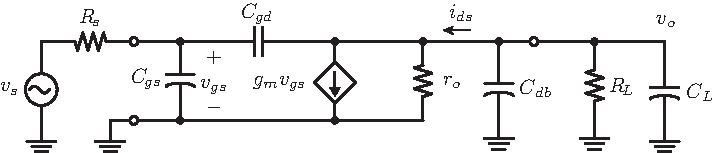
\includegraphics[scale=1]{cs_amp_ac_caps}
\end{center}
\caption{The complete schematic of a common source amplifier including $C_L$ and $C_{db}$.} \label{fig:cs_amp_ac_caps2}
\end{figure}

Let's revisit the common-source amplifier.  As before, we drive it with a source of impedance $R_s$ and load it with $R_L$, as shown in Fig.~\ref{fig:cs_amp_ac_caps}.  We can conveniently add a load capacitance as it appears in parallel with $C_{db}$ and does not complicate the circuit. Since it's not obvious if there's a ``dominant node" in the circuit, we must step through each capacitor and find the equivalent resistance seen by each one. 



\subsection{OCTC:  $R_{C_{gs}}$}

\begin{figure}[tb]
\begin{center}
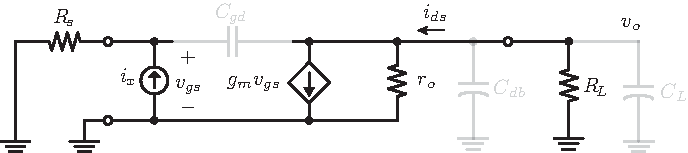
\includegraphics[scale=1]{cs_amp_ac_caps_Cgs}
\end{center}
\caption{Equivalent circuit for calculation of $R_{C_{gs}}$ for OCTC analysis.} \label{fig:cs_amp_ac_caps_Cgs}
\end{figure}

Let's focus on $C_{gs}$, as shown in Fig.~\ref{fig:cs_amp_ac_caps_Cgs}. Note that we open-circuit all the capacitors and replace $C_{gs}$ with a current source to find the equivalent resistance seen by $C_{gs}$.
 Since $C_{gd}$ is open, there's no path from the input to output, and the resistance seen by $C_{gs}$ is simply $R_s$:
%
\begin{equation}
	{R_{C_{gs}}} = R_{s}
\end{equation}


\subsection{OCTC:  $R_{C_{gd}}$}

\begin{figure}[tb]
\begin{center}
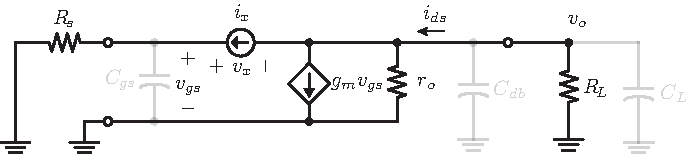
\includegraphics[scale=1]{cs_amp_ac_caps_Cgd}
\end{center}
\caption{Equivalent circuit for calculation of $R_{C_{gd}}$ for OCTC analysis.} \label{fig:cs_amp_ac_caps_Cgd}
\end{figure}
 
Next we focus on $C_{gd}$ as shown in Fig.~\ref{fig:cs_amp_ac_caps_Cgd}.  We open-circuit all the capacitors and replace $C_{gd}$ with a current source to find the equivalent resistance seen by $C_{gd}$.  Let $R_L' = R_L || r_o$.  Since the current $i_x$ flows into the input, we have to be a bit more careful in finding the equivalent resistance seen by $C_{gd}$:
%
\begin{equation} 
	{i_x} = -{g_m}{v_{gs}} - \frac{{{v_d}}}{{R_L'}} = -{g_m}{v_{gs}} - \frac{{{v_{gs}}-{v_x} }}{{R_L'}} 
\end{equation}
%
Using:
\begin{equation} 
	{v_{gs}} =  {i_x}R_{s} 
\end{equation}
%
We find:
%
\begin{equation} 
	{R_{C_{gd}}} = \frac{{{v_x}}}{{{i_x}}} = R_{s}(1 + {g_m}R_L') + R_L' 
\end{equation}



\subsection{OCTC:  $R_{C_{db}}$}

\begin{figure}[tb]
\begin{center}
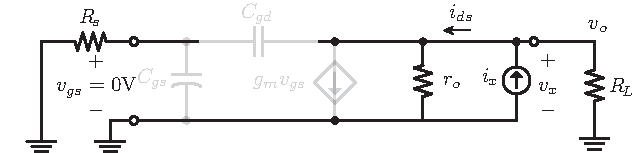
\includegraphics[scale=1]{cs_amp_ac_caps_Cdb}
\end{center}
\caption{Equivalent circuit for calculation of $R_{C_{db}}$ for OCTC analysis.} \label{fig:cs_amp_ac_caps_Cdb}
\end{figure}

Finally we have $C_{db}$ (and $C_L$), shown in Fig.~\ref{fig:cs_amp_ac_caps_Cdb}. To calculate the resistance seen by $C_{db} + C_L$, note that with $C_{gd}$/$C_L$ eliminated (open), there's no voltage at the input, so $v_{gs} = 0$V and so $g_m V_{gs} = 0$A and the current generator is also an open.  So by inspection:
%
\begin{equation}
	{R_{{C_{db}}+C_L}} = R_L'
\end{equation}
%




\subsection{Applying OCTC to CS Amplifier}


Putting all of our results together, we have the sum of the time constants:
%
\begin{equation} 
	{\tau _H} = R_s{C_{gs}} + \left( {R_s(1 + {g_m}R_L') + R_L'} \right){C_{gd}} + R_L'{C_L}
\end{equation}
%
which can be re-written as:
\begin{equation} 
	{\tau _H} = R_s{C_{gs}} + R_s(1 + {g_m}R_L'){C_{gd}} + R_L'{C_{gd}} + R_L'{C_L} 
\end{equation}
%
or approximately:
\begin{equation} 
	 \approx R_s\left( {{C_{gs}} + (1 + {g_m}R_L'){C_{gd}}} \right) + R_L'\left( {{C_{gd}} + {C_L}} \right)
\end{equation}
%
Note that the first term is the same as the time constant from input port resulting from the Miller equivalent circuit.  The second term is the time constant contribution from the output port of the Miller equivalent circuit.  This result matches Eq.~\ref{eq:pole_almost_exact} when we account for $C_L$ and $C_{db}$, which we neglected earlier.
 



\subsection{Practical Approach}

While the method of OCTC works very well for circuits with a dominant pole, it's cumbersome to use if there are many capacitors.  In practice, we can estimate the value of the dominant pole by finding the dominant $RC$ time constants and neglecting others.  If this $RC$ time constant is larger than all others ($100\times$ for example), it's a good approximation to neglect the others and only use one time constant. Many amplifiers are \textit{designed} to have a dominant ``high Z" node for stability reasons, and so we can quickly estimate the bandwidth in these cases.  As you will learn, even if such a ``high Z" node does not exist, we create it by adding capacitance intentionally to \textit{compensate} the frequency response.  This concept will be introduced when we talk about feedback and stability in operational amplifiers, see Section~\ref{sec:opamp_stability}.
 

\section{Chapter Summary}

This chapter introduced several techniques to estimate the frequency response of an amplifier, from ``inspection" style analysis when nodes are independent, to the Miller Theorem and approximation and finally the method of the OCTC, including the simpler version of just estimating the dominant time constants and ignoring others.  Many approximations were made because in doing hand analysis (and design) we are interested in gaining insight into circuit behavior, rather than getting precise answers.  We have full blown circuit simulation tools when we desire accuracy, but often numerical techniques don't lead to insights for design.  This is why we need both hand analysis and computer simulation to design circuits.




